\documentclass[]{article}
\usepackage{amsmath}
\usepackage{graphicx}

%\renewcommand{\familydefault}{\sfdefault}

%opening
\title{Math 45 Final Project: Calculating the Maximum Altitude Attainable by a Rocket in the Earth's Atmosphere}
\author{Kaveh Pezeshki, Aubrey Egerter, Katie Partington, Jose Suarez}

\begin{document}

\maketitle

\section{Introduction and Constraints}

\hspace{0.2in}\textbf{Slide 2} 

\hspace{-0.2in}In this project, we aimed to optimize the dimensions of a rocket to obtain is maximum altitude. We immediately noted that a rocket's altitude is dependent on multiple factors: the mass of the rocket, its fuel capacity, how fast, in terms of velocity and mass per unit time, it can eject the fuel, as well as the drag on the rocket. There would be an upward force due to thrust, and downward force due to its mass.

\textbf{Slide 3}

However, rocket design is immensely complex, and simplifying assumptions would be necessary. While detailed assumptions in terms of the engine design, atmospheric composition, and other factors are described in the relevant sections of this paper, the largest simplification made is for the rocket to be a cone with a given height, where we vary its vertex angle. This brings immediate consequences: we predict that drag will be lower with a smaller angle, but a smaller angle will reduce the volume of the rocket and therefore its fuel storage capacity.

The rocket is constrained to be a cone, with a  height $h$ and vertex angle $\theta$. The former variable is fixed: our justification for this is that height is a large constraining factor for rocket production today. Assembly facilities are limited by the height of their roof. The rocket is also not entirely composed of fuel: there are control systems and engine components that need to be included in the model. Therefore we created the following set of parameters, based on the model of a rocket rising through the Earth's atmosphere against gravity, which is assumed to be constant, and drag.

\textbf{Slide 4}

\begin{center}
	\begin{tabular} {c l l}
		Parameter Name & Description & Type \\
		$\theta$ & Vertex angle of the rocket cone & Optimized\\
		$h$ & Height of the rocket & Dependent Variable\\
		$\sigma$ & Air density (assumed to be constant) & Constant parameter\\
		$\phi$ & Fuel density & Constant parameter\\
		$\gamma$ & Fuel ejection rate from the rocket & Constant parameter\\
		$u$ & Speed differential between ejected fuel and rocket & Constant parameter\\
		$\alpha$ & Drag coefficient (to be later defined) & Calculated constant parameter
	\end{tabular}
\end{center}


\textbf{Slide 5}

We see the following force diagram for the rocket in figure \ref{forces}.

\begin{figure}[h]
	\begin{center}
		\caption{Rocket Force Diagram}
		\label{forces}
		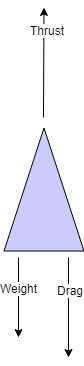
\includegraphics[scale=0.5]{forces.png}
	\end{center}
\end{figure}


We therefore need to calculate the magnitude of the drag force on the rocket. The weight force is known: $F_{weight} = Mg$.

\textbf{Slide 6}

As drag force is a complex phenomenon, we built our physical demonstration around our model of it. In the tray we have marbles, representing air particles, as well as a wooden triangle representing the ship. While this is a 2D approximation of our 3D model, it demonstrates the same characteristics that we use to model drag.

As we move the ship through the marble field, the marbles bounce off of the side of the ship: some momentum of the ship is imparted onto the marbles, which averages into a constant drag force.

\newpage
\section{Calculating Drag Force}

\textbf{Slide 7}

We abstract the atmosphere as a collection of equally spaced point masses at rest with density $\sigma$, and without any inter-particle forces. Additionally, we assume that there are enough of these particles that the rocket's collisions will generally be continuous. While particles within the atmosphere are not at rest, there's generally little to no net movement such that the vector sum of the motion of all particles within a constrained area of the atmosphere is approximately zero. We assume that all collisions are elastic, and that atmospheric pressure is constant, an assumption that vastly simplified our calculations.


If the rocket is moving at some velocity $\vec{v_{r}}$, then the air particles are similarly approaching the rocket in its own rest frame at some velocity $\vec{v_0}$, equal in magnitude to $\vec{v_{r}}$ and, after bouncing off elastically, they lose some momentum in the $\hat{v_0}$ direction. As we know that angle of incidence is equal to the angle of reflection, we can calculate this velocity change. Additionally, as cones are entirely symmetrical about their axis of symmetry, and the particle field is uniform, we know that all momentum change not in the $\hat{v}$ direction will be `canceled out' in its effect on the rocket by particles colliding on the opposite point of the cone about its axis of symmetry. The geometry of the collision can be seen in figure \ref{collision}.

\begin{figure}[h]
	\begin{center}
		\caption{Collision Geometry of the Rocket and Atmospheric Particle}
		\label{collision}
		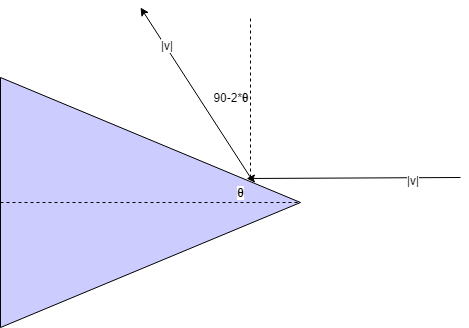
\includegraphics[scale=0.5]{collision.png}
	\end{center}
\end{figure}


Therefore for a single particle of mass $m$ the momentum change is:
\begin{center}
	\begin{align*}
	\Delta P &= m\times (v-v\sin(90-2\theta)) \\
	\Delta P &= mv\times(1-\cos(2\theta)) .
	\end{align*}
\end{center}

We can also find the mass of particles the rocket passes through in some time $\delta t$:

\begin{center}
	\begin{align*}
	m &= \text{air volume rocket moved through}\times \text{density of air} \\
	m &= \pi r^2 v \Delta t \times \sigma \\
	m &= \pi h^2 \tan^2(\theta) v \Delta t \sigma .
	\end{align*}
\end{center}

And substitute this expression into the expression for momentum change:

\begin{center}
	\begin{align*}
	\Delta P &= mv\times(1-\cos(2\theta)) \\
	\Delta P &= \pi h^2 \tan^2(\theta) v \Delta t \sigma \times v\times(1-\cos(2\theta)) \\
	\Delta P &= v^2 \Delta t \sigma \pi h^2 \tan^2(\theta) (1-cos(2\theta)) \\
	\Delta P &= \alpha v^2 \Delta t \text{  where $\alpha$ is the drag coefficient} \\
	\frac{\Delta P}{\Delta t} &= \alpha v^2 \\
	F_{drag} &= \alpha v^2 \text{  taking the limit $t\rightarrow 0$} .
	\end{align*}
\end{center}

We have now found the drag force via a first-order differential equation.


\section{Calculating the Rocket's Motion}
\textbf{Slide 8}

We can now find the rocket's motion via considering conservation of momentum. The below diagram illustrates fuel ejection from the rocket at times $t$ and $t+\Delta t$. The mass of the rocket is $M$, and the mass of the fuel ejected over the interval is $\Delta m$. The velocity of the rocket is $V$, its gain in velocity is $\Delta V$, and the speed differential between it and the fuel is $V+\Delta V$.

This model makes the assumption that fuel is always ejected at the same rate and velocity, and that it is always ejected in direction $\hat{V}$.

\begin{figure}[h]
	\begin{center}
		\caption{Momentum Conservation in the Rocket-Fuel System}
		\label{momentum}
		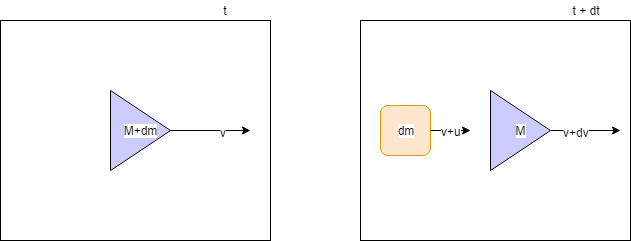
\includegraphics[scale=0.6]{momentum.png}
	\end{center}
\end{figure}

We can now write expressions for the momentum of the system at the two times

\begin{center}
	\begin{align*}
	P_{t} &= V(M+\Delta m) \\
	P_{t+\Delta t} &= M(V + \Delta V) + \Delta m (V+u) .
	\end{align*}
\end{center}

We can write this in terms of the applied force

\textbf{Slide 9}

\begin{center}
	\begin{align*}
	\Delta P &= P_{t+\Delta t} - P_{t} \\
	\Delta P &= M(V + \Delta V) + \Delta m (V+u) - v(M+\Delta m) \\
	\Delta P &= M\Delta V + u\Delta m \\
	\frac{\Delta P}{\Delta t} &= M\frac{\Delta V}{\Delta t} +  u\frac{\Delta m}{\Delta t} \\
	F_{external} &= M \frac{dV}{dt} + u \frac{dm}{dt} \text{  taking the limit $t\rightarrow 0$} .
	\end{align*}
\end{center}

We can now isolate $\frac{dV}{dt}$ and express $F_{external}$ in terms of the previously calculated drag and weight, implementing previously-defined constants.

We see that:

\begin{center}
	\begin{align*}
	M(t) &= M_0 - \gamma t . \\
	F_{weight} &= Mg .
	\end{align*}
\end{center}

Therefore:

\begin{center}
	\begin{align*}
	\frac{dV}{dt} &= \frac{u \frac{dm}{dt}}{M} - \frac{F_{external}}{M}  \\
	\frac{dV}{dt} &= \frac{u\gamma}{M_0 - \gamma t} - \frac{(M_0 - \gamma t)g + \alpha V^2}{M_0 - \gamma t} \\
	\frac{dV}{dt} &= \frac{u\gamma - \alpha V^2}{M_0 - \gamma t} - g .
	\end{align*}
\end{center}

\textbf{Slide 10}

We now have a differential equation describing the velocity of the rocket as a function of time. We also have a differential equation describing its altitude:

\begin{center}
	\begin{align*}
	\frac{dS}{dt} &= V .
	\end{align*}
\end{center}

As the former equation has no closed-form solution, a numerical approximation can be done via Euler's method. The same set of timesteps can be used in a second application of Euler's method to calculate altitude as a function of time.

\section{Solution Existence}

\textbf{Slide 11}

With reference to the physical implications of our solution, it is clear that the solution only exists during $0 \le t < t_{f}$, where $t_f$ occurs when there is no fuel left in the rocket. We can calculate $t_f$, with $volume_{other}$ referencing the volume of the rocket consumed by the payload, control systems, and other non-fuel entities:

\begin{center}
	\begin{align*}
	t_f &= \frac{M_{fuel}}{\gamma} \\
	t_f &= \frac{\phi volume_{fuel}}{\gamma} \\
	t_f &= \frac{\phi (volume_{rocket} - volume_{other}) } {\gamma} \\
	t_f &= \frac{\phi (\pi r^2 \frac{h}{3} - volume_{other}) } {\gamma} \\
	t_f &= \frac{\phi (\pi h^2 \tan^2(\theta) \frac{h}{3} - volume_{other}) } {\gamma} . \\
	\end{align*}
\end{center}

There is another condition for physical existence present in the solution. Drag is always assumed to be opposite in direction to that of the rocket's initial motion. However, the drag force will be upward when $V$ is negative. Therefore the solution is only valid until the point where $V$ experiences its first negative value. This forces a partial redefinition of our problem: we find not the maximum altitude, but the altitude at which the rocket produces no more thrust.

\section{Euler's Method Approximation}

\textbf{Slide 12}

A python script was written to approximate velocity and altitude via Euler's method, which then exported data to a .csv file which can be analyzed via Excel. This script is available in a GitHub repository\footnote{https://github.com/Arcturus314/math45\_final}.


 Specifically, the algorithm used was, with $\Delta t$ the timestep:

\begin{center}
	\begin{align*}
	V_{t+\Delta t} &= V_{t} + \frac{dV_{t}}{dt}\times \Delta t \\
	S_{t+\Delta t} &= S_{t} + V_{t}\times \Delta t .
	\end{align*}
\end{center}

With the luxury of computer automation on our side, and the relative simplicity of calculating $\frac{dV}{dt}$, we found that no timestep lower than $\Delta t = 0.0001$ offered a distinguishable output.

\section{Establishing Parameter Values}

\textbf{Slide 13}

We then needed to find reasonable parameters for our rocket model. Data for all necessary constants are not publically available for the single-stage rocket approximated by our model. We therefore assembled a reasonable set of parameter values from various rockets. 

\begin{center}
	\begin{tabular} {l l} 
		Parameter & Value \\
		\hline
		height & 60 $m$ size of Falcon 9 http://www.spacex.com/falcon9\\
		fuel density & 600 $kgm^{-3}$ averaged between liquid hydrogen and oxygen densities\\
		fuel ejection rate & 56100 $kg s^{-1}$ fuel ejection rate of Saturn V first stage \\ & \small https://www.theatlantic.com/technology/archive/2016/03/the-saturn-v-in-elephants/475314/ \normalsize\\
		air density & 1.225 $kg m^{-3}$ https://www.omnicalculator.com/physics/air-density\\
		other volume & 1200 $m^3$ http://www.spaceflightinsider.com/hangar/falcon/\\
		other mass  & 25600$kg$  http://www.spaceflightinsider.com/hangar/falcon/ \\
		fuel ejection speed & 3000 $ms^{-1}$ \\ &https://physics.stackexchange.com/questions/191949/velocity-of-rocket-exhaust
	\end{tabular}
\end{center}
	
	
\textbf{Slide 14}

Substituting these values into the Euler's method approximator produced plots for $\theta = \frac{\pi}{20}$ as seen in figure \ref{velalt}.

Velocity appears to roughly maintain a constant derivative, although with minor positive curvature, due to the interaction between thrust, mass loss, and increasing drag force. As its derivative decreases near 50 seconds the velocity begins to approach a positive steady state, the point at which drag force and mg is roughly equal in magnitude to thrust. The plot ends at the point when the rocket has run out of fuel.

The altitude graph appears as expected given its derivative: altitude increases roughly quadratically as a function of time, until the velocity begins to reach its steady state, at which point altitude increases linearly.


\begin{figure}[h]
	\centering
	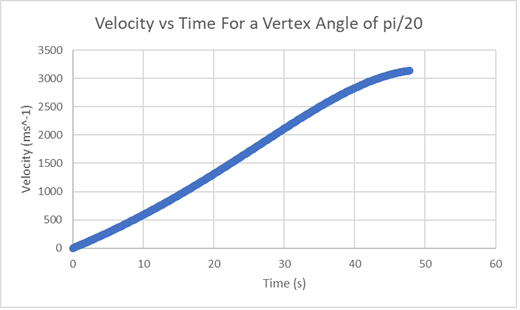
\includegraphics[width=0.495\textwidth]{velocity.png}
	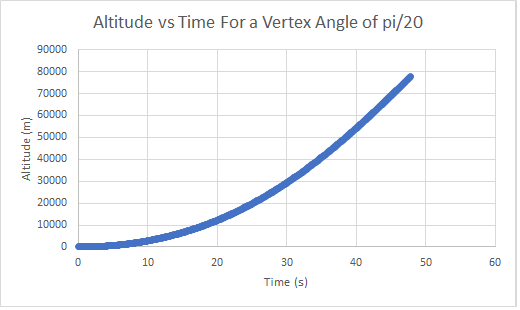
\includegraphics[width=0.495\textwidth]{altitude}
	\caption{Velocity and Altitude over time for $\theta = \frac{\pi}{20}$}.
	\label{velalt}
\end{figure}


\section{Optimizing Nose Cone Angle}

\textbf{Slide 15}

We then used the previously-written Python script to generate maximum altitudes for vertex angles $0<\theta<\frac{\pi}{2}$. This plot can be seen in figure \ref{optimization}.

\begin{figure}[h]
	\begin{center}
		\caption{Plotting Maximum Altitude against Vertex Angle}
		\label{optimization}
		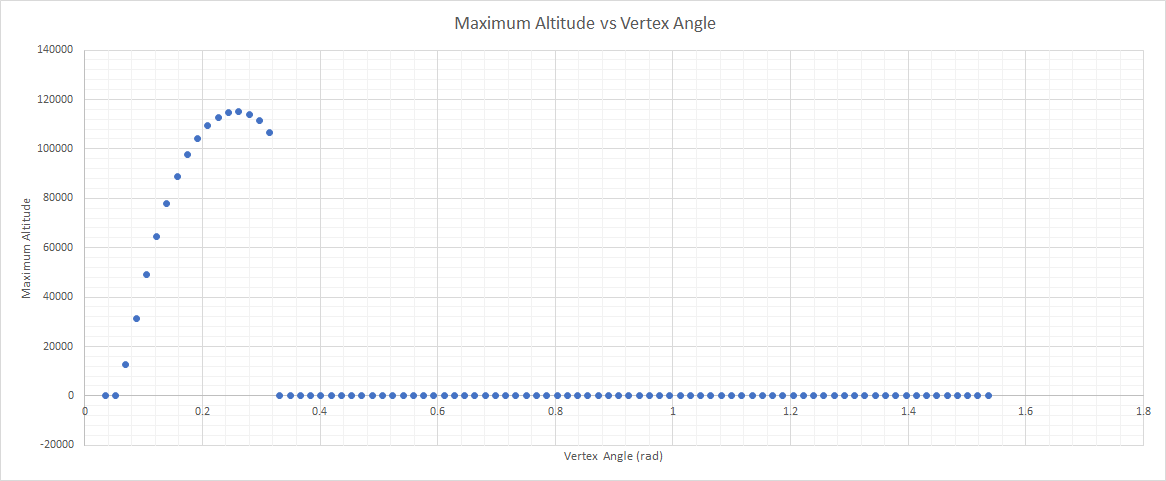
\includegraphics[scale=0.5]{optimization.png}
	\end{center}
\end{figure}

The maximum altitude occurs at a nosecone angle of $\theta = 0.261799 rad$, with an altitude of 115km. The smallest nosecone angle at which the rocket gains altitude occurs when the cone has a large enough volume to fit the `other' components, and the angle for which the rocket fails to ascend near 0.3 radians occurs when the mass of the laden rocket produces a weight larger than its thrust.


\section{Analysis}
\textbf{Slide 16}

Our obtained result is reasonable. While our rocket included only one stage, it passed the Karman line at 100km \footnote{http://www.iop.org/resources/topic/archive/space/}, which is commonly considered the boundary between air and space, as it is the point at which the air density is too low for flight \footnote{http://www.messagetoeagle.com/what-is-the-karman-line/}. As the rockets from which model parameters were derived all passed the Karman line, we see that our model produced reasonable values.

\textbf{Slide 17}

However, there are many simplifications inherent in our model, and therefore, many characteristics that could be improved. In particular, the accuracy of our model would be increased if the expression for drag included a variable height-dependent air density term. Drag was the limiting factor in acceleration of the rocket once it had reached reasonable speed, and as such more accurate results would be obtained if air density was more precisely modeled. Similarly, gravity is variable as a function of height: implementing this into our model would further increase accuracy.

Finally, it would be worthwhile to explore other parameterized rocket designs: for example, a classic nosecone-and-cylinder design as seen in current high-altitude rockets. However, the presence of multiple parameters would lead to computational difficulty in identifying the ideal rocket design.

\end{document}


